\chapter{Preprocessing image}
\section{Problem}
The propriety of an algorithm or a program often based on a good input set. To obtain the good result when applying the automatic classification methods. In this chapter, we suggest the algorithm preprocessing image. With the input images contains the parts of insect and an unexpected object, specifically yellow grid (Fig \ref{fig:Figure_1}), we need remove the yellow grid to have only insect and just keep the insect.
\begin{figure}[h!]
\centering
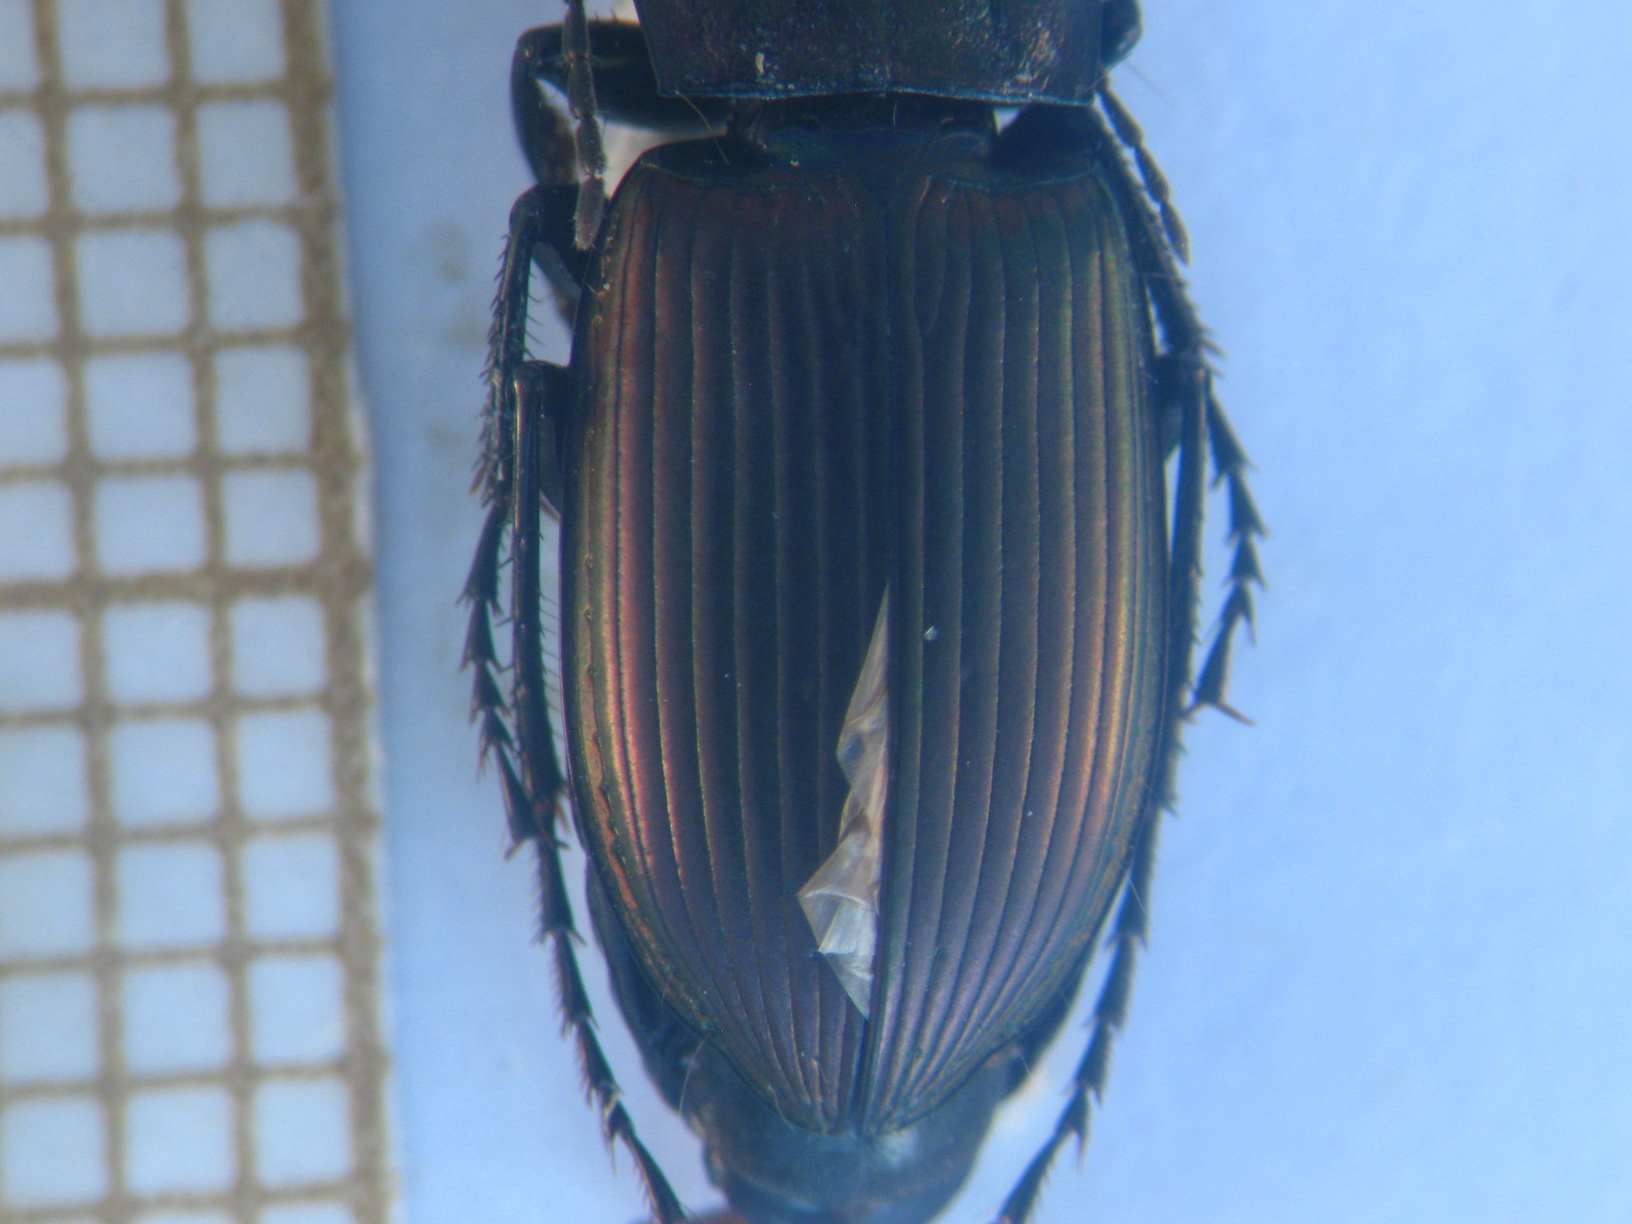
\includegraphics[width=0.5\textwidth]{./images/input}
\caption{An input image with yellow grid}
\label{fig:Figure_1}
\end{figure}\\
\section{Analysis}
Each input image contains the two objects: the part of insect and the yellow grid (called grid). Addition, the grid always stay on the left of image, and the insect can either overlap the grid or not. About the color, we can see three main groups color: the background color, the yellow color of grid and the color of insect. The image is presented in BGR model. So, the color at each pixel must be combine among three values (blue, green, red). If we process the image in BGR model, the algorithm may be complex. While, the HSV model just has a channel to present the value of color and each color has a clear range. We can apply this property for detecting and removing the gird.\\
The analysis system is constructed from two main stages: finding the limit point of grid, replacing the yellow point from the begin to the limit point.
\section{Method}